\documentclass{beamer}

\usepackage{graphicx}
\usepackage[english]{babel}
\usepackage{array}

\hypersetup{pdfstartview={Fit}}
\setbeamertemplate{navigation symbols}{}
\newcolumntype{P}[1]{>{\centering\arraybackslash}p{#1}}

\AtBeginSection[]
{
  \begin{frame}<beamer>{Outline}
    \tableofcontents[currentsection, currentsubsection, hideallsubsections]
  \end{frame}
}

\begin{document}

% ---------------------------------------------------------------------
%   Title slide and table of contents
% ---------------------------------------------------------------------

\title[LOD] {Linked Open Data at Universities}
\subtitle {A case study concerning students}
\author[Author, Haller] {Kevin Haller}
\date[2016] {Seminar Work, 2016}
\subject{Computer Science}

\frame{\titlepage}

\begin{frame}
\frametitle{Table of Contents}
\tableofcontents[hideallsubsections]
\end{frame}

% --------------------------------------------------------------------------------------------
%  Introduction
% --------------------------------------------------------------------------------------------

\section[Introduction]{Introduction}
\begin{frame}
\frametitle{Introduction}
\end{frame}

\subsection[Research questions]{Research questions}
\begin{frame}
\frametitle{Research questions}
\begin{description}
	\item[RQ1:] \textit{What are best practices regarding the applicability of Linked Open Data in university
settings?}
	\item[RQ2:] \textit{What are the major benefits and challenges for students if certain university resources
are published as Linked Open Data and which needful use cases can result out of this from the
perspective of the students?}
	\item[RQ3:] \textit{What are major challenges for the implementation of a Linked Open Data solution?}
	\item[RQ4:] \textit{How would a prototypical implementation of a publication framework based on Linked Open
Data look like?}
\end{description}
\end{frame}

% --------------------------------------------------------------------------------------------
%  Related works
% --------------------------------------------------------------------------------------------
\section[Related Work]{Related Work}


% --------------------------------------------------------------------------------------------
%  Result: Case study
% --------------------------------------------------------------------------------------------

\section[Benefits and challenges]{Benefits and challenges of using Linked Open Data at universities}
\begin{frame}
\frametitle{Benefits and challenges}
\begin{description}
	\item[Case study] were conducted aimed to answer the research question: \textbf{\textit{RQ2}} and \textbf{\textit{RQ3}}.
\end{description}
\end{frame}

\subsection[Methodology]{Methodology}
\begin{frame}
\frametitle{Methodology}
\begin{description}
	\item[Exploration of the state of the art] including case studies related to Linked Data applied to universities. 
	\item[5 semi-structured interviewees] with students and people affiliated with student affairs were conducted.
	\begin{itemize}
		\item The interviews followed a questionnaire.
		\item The interviews were conducted in teams of two researcher. One \textit{\textbf{moderator}} and one \textit{\textbf{logger}}, who had the task to collect data by writing valuable contributions onto a logging sheet.
	\end{itemize}
\end{description}
\end{frame}

\subsection[Interviewees background]{Interviewees background}
\begin{frame}
\frametitle{Interviewees background}
\framesubtitle{The interviewees were asked about their background.}
\begin{table}[h]
	\small
	\begin{tabular}{| l | c | P{0.9cm} | c | c |}
 		\multicolumn{2}{c}{} & \multicolumn{2}{P{2.25cm}}{Level of expertise (1-5)} \\
 		\hline
		ID & Assignment & ICT & LOD & Date of interview \\
		\hline
		A  & student representative & 3 & 1 & 24.11.2015\\
		B & teaching \& administration & 5 & 2 & 03.12.2015\\
		C & teaching \& administration & 5 & 1 & 17.12.2015\\
		D & student & 4 & 3 & 12.02.2016\\
		E & student & 4 & 3 & 18.02.2016\\
		\hline
	\end{tabular}
	\label{table:interviewee-background}
\end{table}
\begin{table}[h]
	\footnotesize 
	\begin{tabular}{ c | l  | p{7cm} }
		Value & ICT & LOD\\	
		\hline
		1 & Fundamental & I never heard of Linked Open Data.\\
		2 & Novice & I heard of Linked Open Data, but never used it.\\
		3 & Intermediate & I used Linked Open Data in a not intense way. E.g. as part of a workshop or home project.\\
		4 & Advanced & I used Linked Open Data in a practical project.\\
		5 & Expert & I used Linked Open Data in several practical projects and consider myself an expert in Linked Open Data.\\
	\end{tabular}
	\caption{Scala for level of expertise}
	\label{table:interviews-rating scales}
\end{table}
\end{frame}

\subsection[Use cases and needs]{Use cases and needs}
\begin{frame}
\frametitle{Use cases and needs}

\end{frame}

\subsection[Adoption potential]{Adoption potential}
\begin{frame}
\frametitle{Adoption potential}
The interviewees were asked about their willingness to develop applications based on Linked Open
Data provided by the university.
\end{frame}

% --------------------------------------------------------------------------------------------
%  Result: Technical architecture and challenges
% --------------------------------------------------------------------------------------------

\section[Technical architecture and challenges]{Technical architecture and challenges}
\subsection{Linked Open Data effort at universities}
\begin{frame}
\frametitle{Linked Open Data effort at universities}
	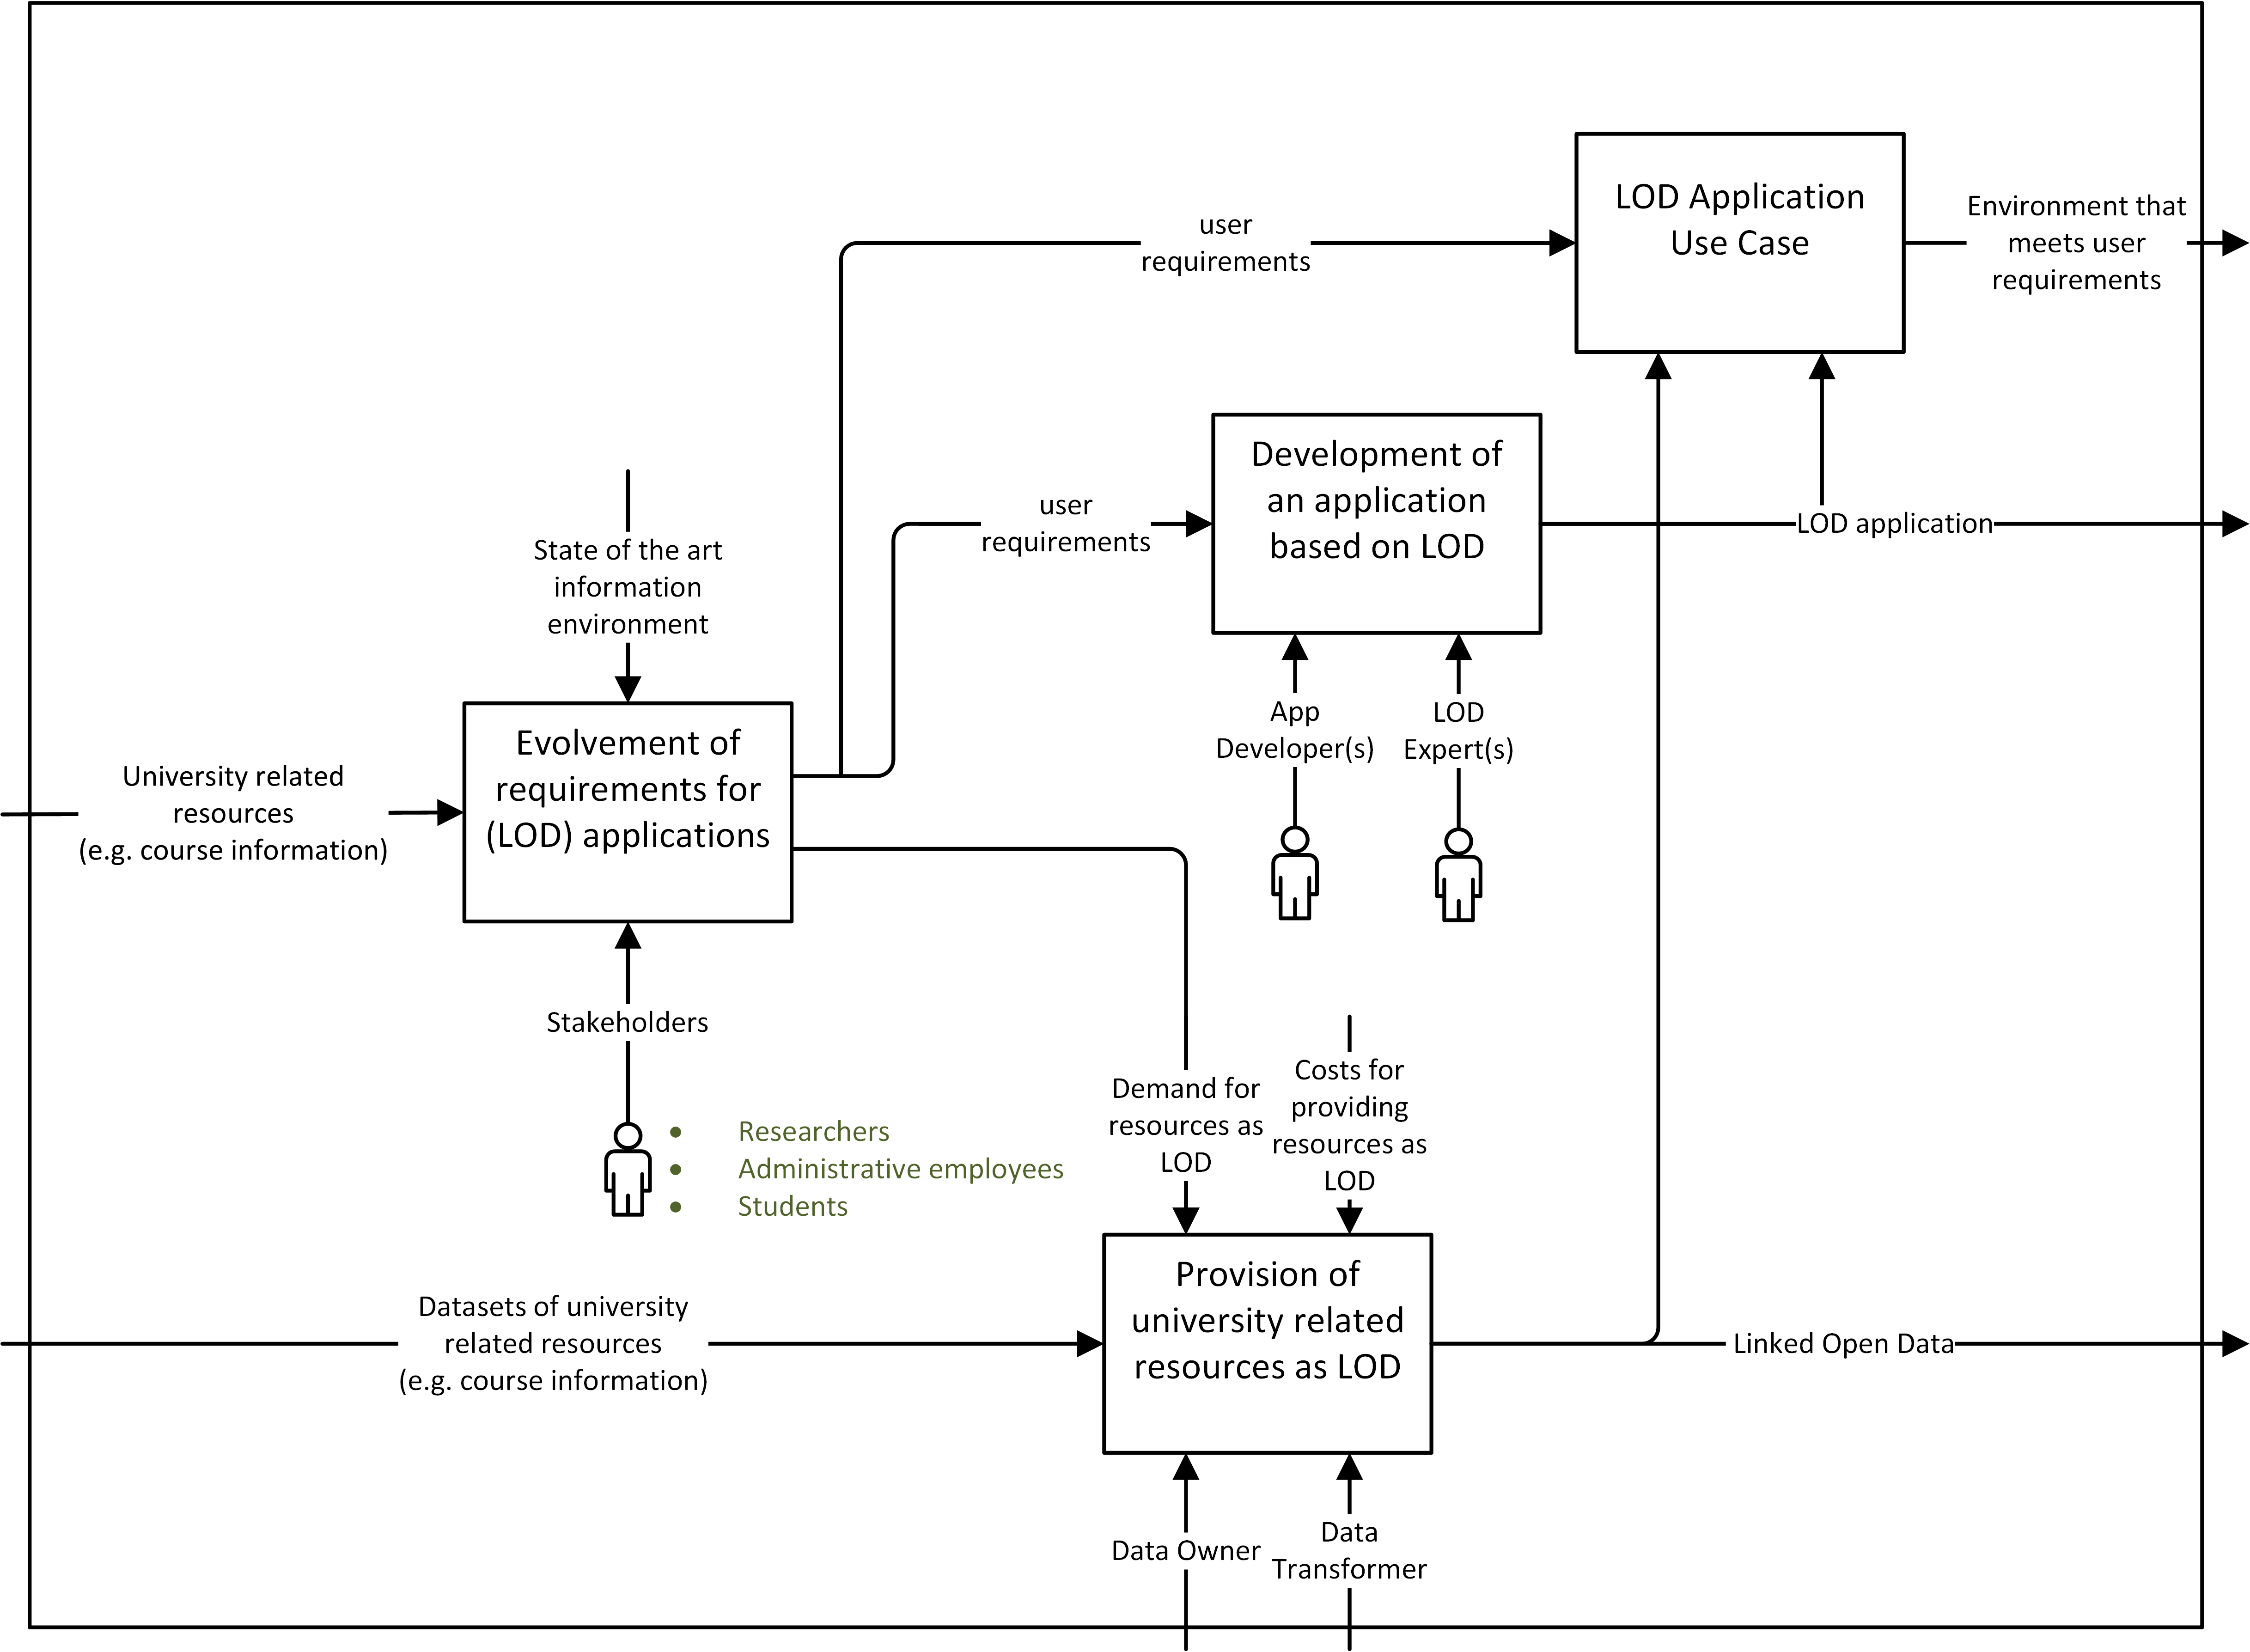
\includegraphics[width=\columnwidth]{../images/technical-architecture/lod_at_tuwien_idef0.png}
\end{frame}
\subsection{Proposal of a technical architecture}
\begin{frame}
\frametitle{Proposal of a technical architecture}
	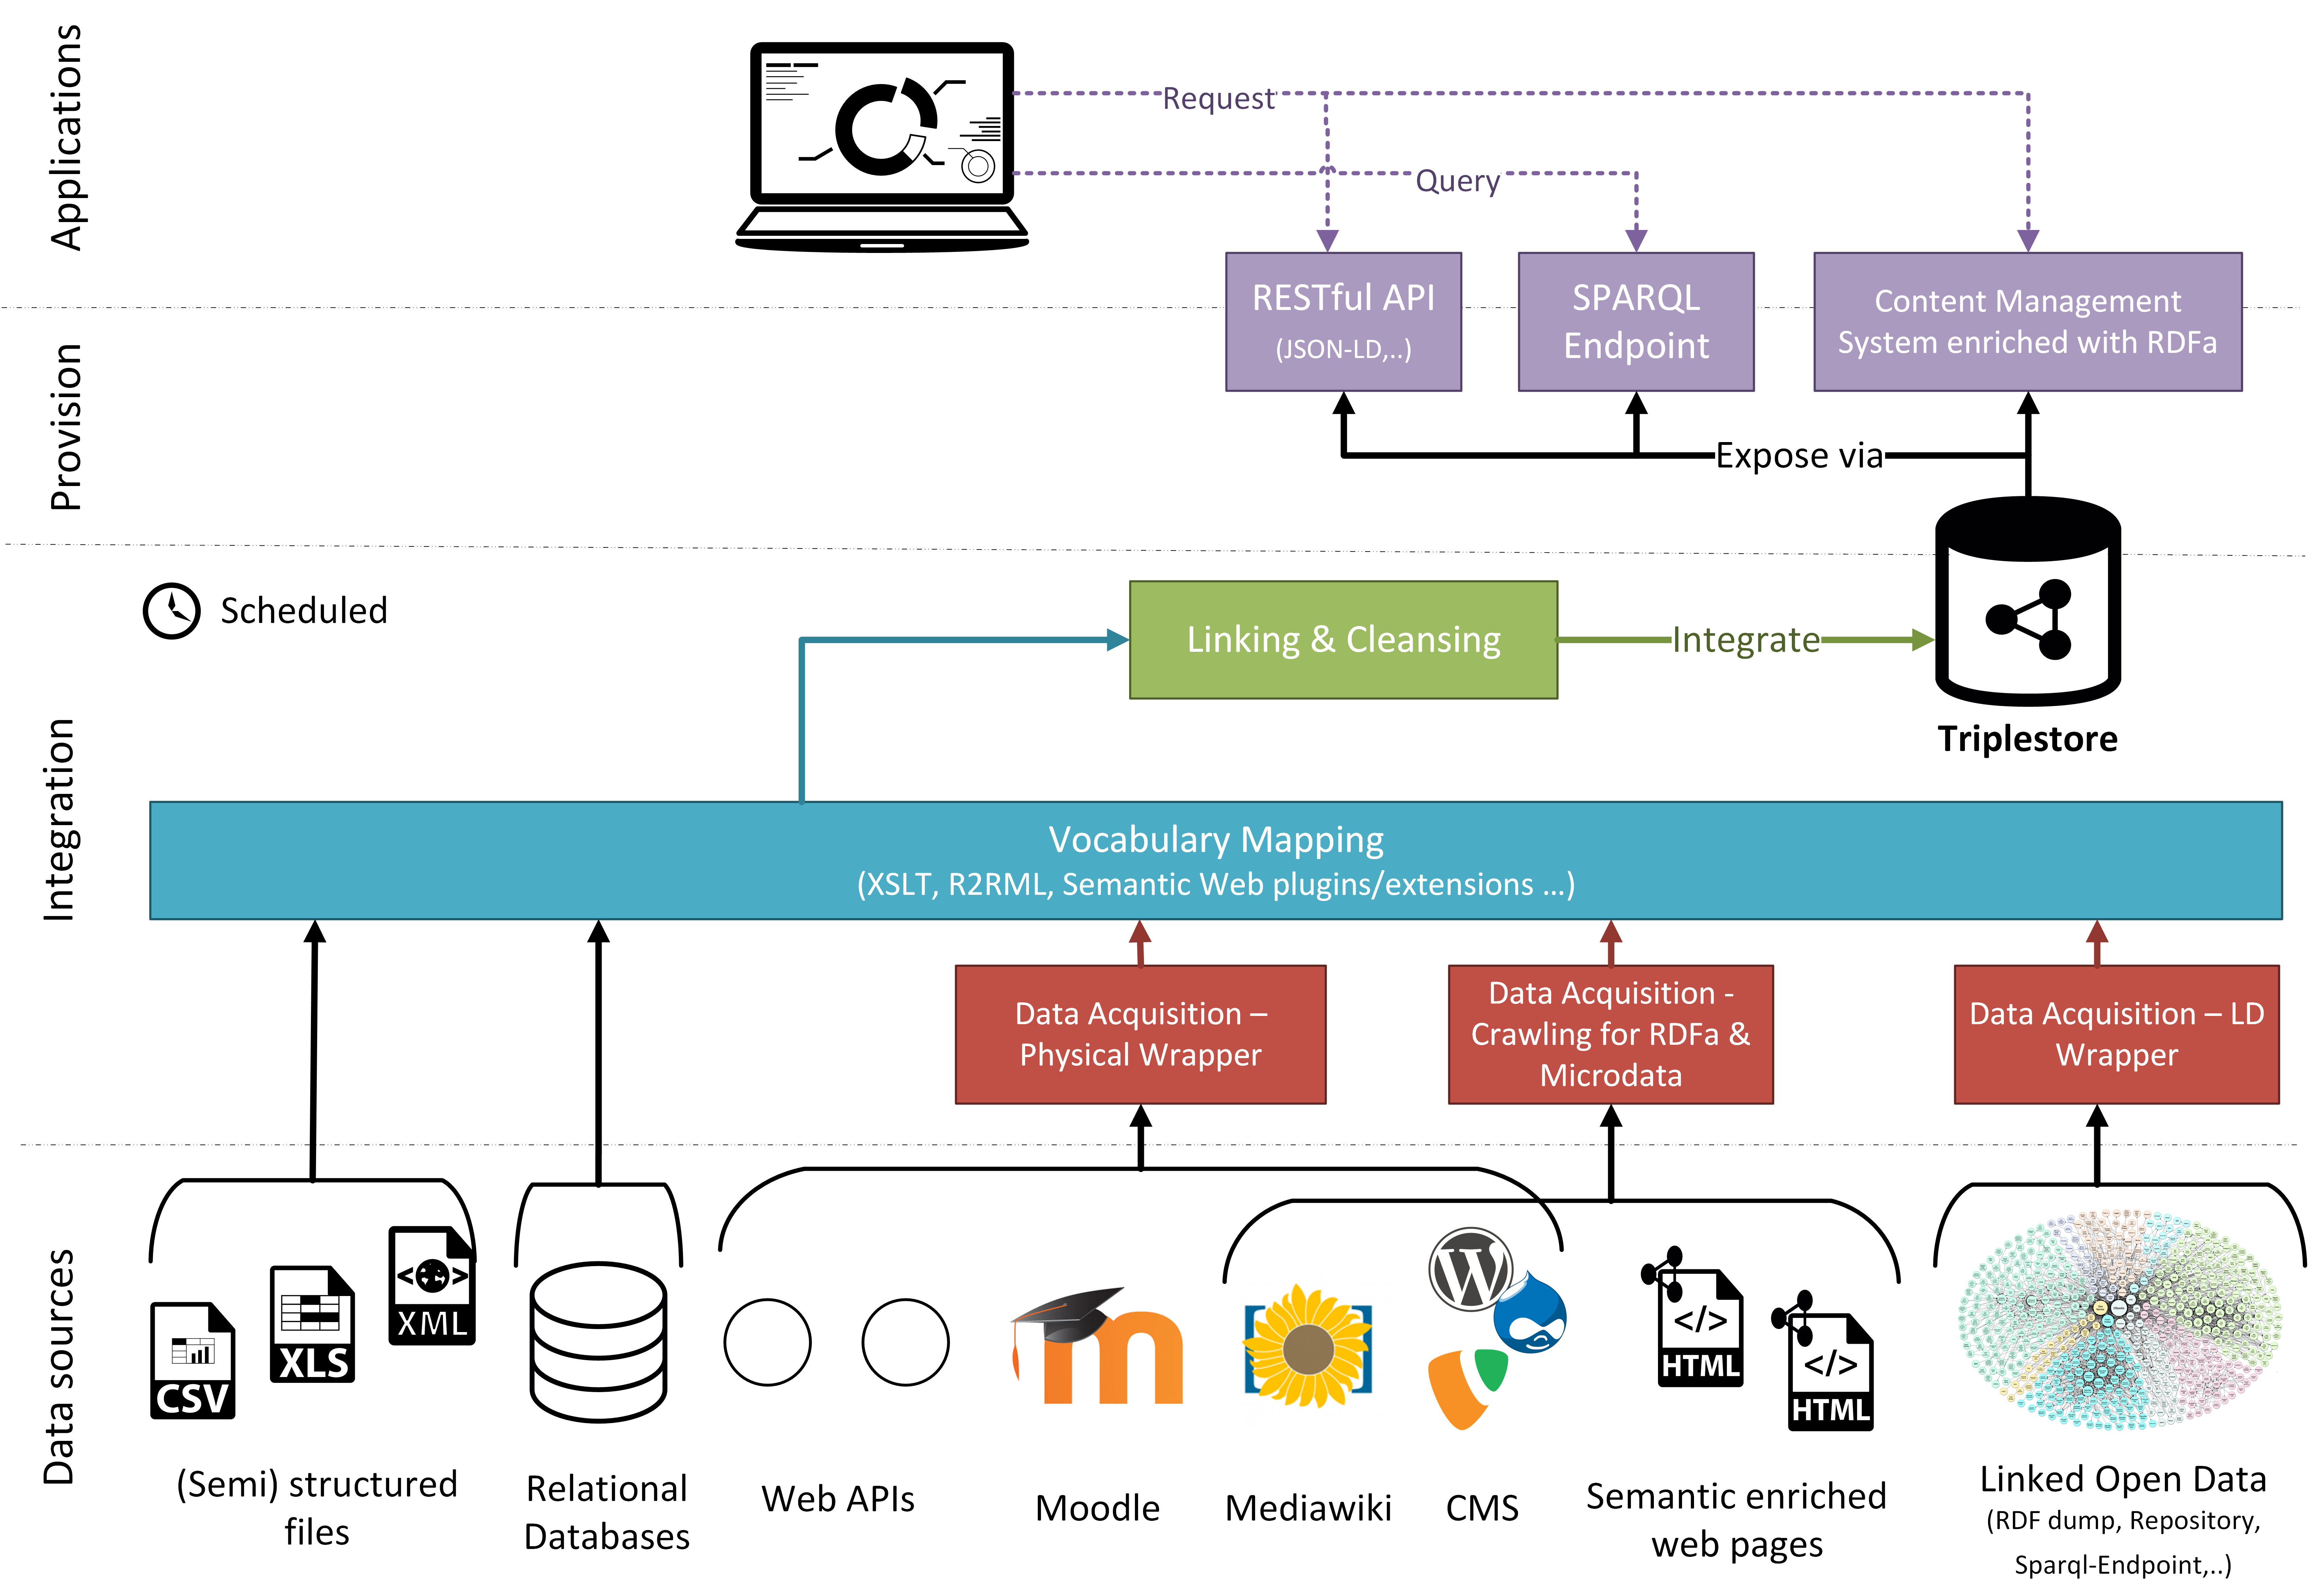
\includegraphics[width=\columnwidth]{../images/technical-architecture/lod_technical_architecture.png}
\end{frame}

\subsection{Challenges}
\begin{frame}
\frametitle{Challenges}
\end{frame}

\subsubsection{Data ownership}
\begin{frame}
\frametitle{Challenges}
\framesubtitle{Data ownership}
\end{frame}

\subsubsection{Data licenses}
\begin{frame}
\frametitle{Challenges}
\framesubtitle{Data ownership}
\end{frame}

\subsubsection{Data freshness}
\begin{frame}
\frametitle{Challenges}
\framesubtitle{Data ownership}
\end{frame}

\end{document}